\item Consider the grid shown
\[
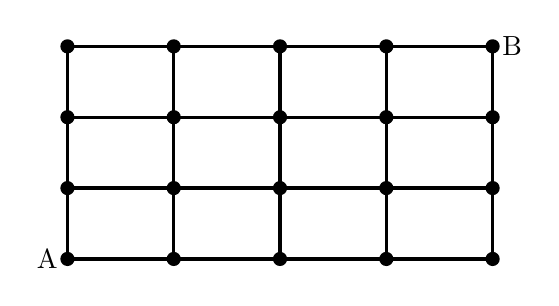
\begin{tikzpicture}[scale=0.9]
    \draw[very thick, xstep=1.5] (0, 0) grid (6, 3);
    \foreach \i in {0, 1.5, ..., 6} {
        \foreach \j in {0, 1, 2, 3} {
            \fill (\i, \j) circle (0.1);
        }
    }
    \node[anchor=east] at (0, 0) {A};
    \node[anchor=west] at (6, 3) {B};
\end{tikzpicture}
\]
Suppose that, starting at the point labeled $A$, you can go one step up or one step to the right at each move. This procedure is continued until the point labeled B is reached. How many different paths from A to B are possible?

Considerar el siguiente ordenamiento lineal
\[ \rightarrow\ \rightarrow\ \rightarrow\ \rightarrow\ \uparrow\ \uparrow\ \uparrow \]
donde $\rightarrow$ indica un movimiento a la derecha y $\uparrow$ indica un movimiento hacia arriba.

Queremos todas las permutaciones únicas de esta secuencia
\[ \frac{7!}{4! * 3!} \]